%Notes by Harsh Mistry 
%Econ 301
%Based on Template From  https://www.cs.cmu.edu/~ggordon/10725-F12/template.tex

\documentclass[twoside]{article}
\setlength{\oddsidemargin}{0.25 in}
\setlength{\evensidemargin}{-0.25 in}
\setlength{\topmargin}{-0.6 in}
\setlength{\textwidth}{6.5 in}
\setlength{\textheight}{8.5 in}
\setlength{\headsep}{0.75 in}
\setlength{\parindent}{0 in}
\setlength{\parskip}{0.1 in}
\usepackage{amsmath,amsfonts,graphicx, color}
\newcounter{lecnum}
\renewcommand{\thepage}{\thelecnum-\arabic{page}}
\renewcommand{\thesection}{\thelecnum.\arabic{section}}
\renewcommand{\theequation}{\thelecnum.\arabic{equation}}
\renewcommand{\thefigure}{\thelecnum.\arabic{figure}}
\renewcommand{\thetable}{\thelecnum.\arabic{table}}
\newcommand{\lecture}[4]{
   \pagestyle{myheadings}
   \thispagestyle{plain}
   \newpage
   \setcounter{lecnum}{#1}
   \setcounter{page}{1}
   
   
%Info Box 
   \begin{center}
   \framebox{
      \vbox{\vspace{2mm}
    \hbox to 6.28in { {\bf Econ 301 - Microeconomic Theory 2
	\hfill Winter 2018} }
       \vspace{4mm}
       \hbox to 6.28in { {\Large \hfill Lecture #1: #2  \hfill} }
       \vspace{2mm}
       \hbox to 6.28in { {\it Lecturer: #3 \hfill Notes By: #4} }
      \vspace{2mm}}
   }
   \end{center}
   
   \markboth{Lecture #1: #2}{Lecture #1: #2}



 
}

\renewcommand{\cite}[1]{[#1]}
\def\beginrefs{\begin{list}%
        {[\arabic{equation}]}{\usecounter{equation}
         \setlength{\leftmargin}{2.0truecm}\setlength{\labelsep}{0.4truecm}%
         \setlength{\labelwidth}{1.6truecm}}}
\def\endrefs{\end{list}}
\def\bibentry#1{\item[\hbox{[#1]}]}

\newcommand{\fig}[3]{
			\vspace{#2}
			\begin{center}
			Figure \thelecnum.#1:~#3
			\end{center}
	}
	
	\graphicspath{ {images/} }

\newtheorem{theorem}{Theorem}[lecnum]
\newtheorem{lemma}[theorem]{Lemma}
\newtheorem{ex}[theorem]{Example}
\newtheorem{proposition}[theorem]{Proposition}
\newtheorem{claim}[theorem]{Claim}
\newtheorem{corollary}[theorem]{Corollary}
\newtheorem{definition}[theorem]{Definition}
\newenvironment{proof}{{\bf Proof:}}{\hfill\rule{2mm}{2mm}}
\newcommand\E{\mathbb{E}}


%Start of Document 
\begin{document}

\lecture{5}{January 17, 2018}{Jean Guillaume Forand}{Harsh Mistry}
\section{Consumer Choice Continued}

\subsection{Optimal consumer choice}
\textbf{\textcolor{red}{In class numbering : 1.1.5}}
\begin{itemize}
\item Consumers choice problem has been reduced to constrained optimization problem (Utility Maximization Problem): 
\[max_{x_1, x_2 \geq 0} \hspace{0.1cm} u(x_1, x_2)  \text{ subject to } p_1 x_1 +  p_2 x_2 \leq m \text{ (PI) }\]
\item Solutions to this problem are \underline{demand functions} \(x_1(p_1m)\) and \(x_2(p_2 m)\)
\item Constraint in (PI) is an inequality constraint
\item We want conditions under which solutions to (PI) are also solutions to the simpler problem 
\[{max}_{x_1,x_2 \geq 0}  u(x_1, x_2) \text{ such that } p_1x_1 + p2x_2 = m \text{ (PE) }\]
\item In other words, under what conditions do solutions to (PI) lie on the budget line. 
\item Result : If consumer preferences are monotone, then any solution to (PE) must be a solution to (PI) 
\item For some non-monotone preferences, consumers can find it optimal not to exhaust her budget.

\begin{center}
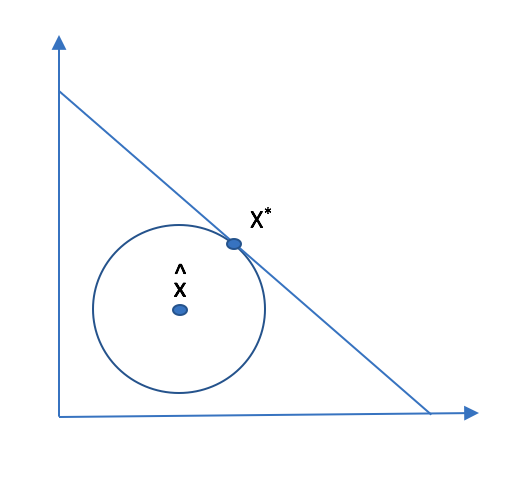
\includegraphics[scale=0.5]{9}
\end{center}

\begin{itemize}
\item \(\hat{x}\) solution to (P.F.)
\item \(x^*\) solution to (P.E.), but not the solution to the original problem, as there is a higher indifference curve that intersects the budget line. 
\end{itemize}
\item If consumers preferences are monotone, (PE) still needs to be solved
\item Use method of Lagrange if \(u\) is differentiable 
\begin{enumerate}
\item Define \underline{Lagrangian}
\[L(x_1, x_2, \lambda) = u(x_1, x_2) + \lambda (m - p_1x_1 - p_2x_2)\]
A function of bundles \(x \in \mathbb{R}^2_+\) and \underline{Lagrange multiplier} \(\lambda \in \mathbb{R}
\)
\item If the solution \(x^*\) to (PE) is such that \(x_1^* x_2^2 \neq 0 \), then it must solve the system of first-order conditions: 
\[\begin{cases}
\frac{d}{dx} L(x_1^* , x_2^*, \lambda) = \frac{d}{dx}  u(x_1^*, x_2^*) - \lambda p_i = 0   \text{ (Li), } i = 1, 2, \ldots \\
\frac{d}{dx} L(x_1^* , x_2^*, \lambda ) = m - p_1 x_1^* - p_2x_2^* = 0 \text { (L} \lambda \text{), }
\end{cases}\]
\end{enumerate}
\item The restriction that \(x_1^*, x_2^* \neq 0\) implies that solution \(x^*\) is \underline{interior} 
\item \(L(1) - L(\lambda)\) is a system of three equations and three unknowns \(x_1^*, x_2^*, \lambda\), and it can be solved in special cases.  
\item Substitute out \(\lambda\) by using (LI) and (L2) 
\[\frac{\frac{d}{dx} u(x_1^*, x_2^*)}{\frac{d}{dx} u(x_1^*, x_2^*) } = \frac{p_1}{p_2} \text{ (MRS) - Marginal rate of exhance}\]
Consumers Marginal rate of substitution : rate at which consumers are wiling to exchange good 2 against  additional units of  good 1  
\item Let \(x^*\) denote consumers with level from \(x^*\) 
\[u(x_1^*, x_2^*) - u^*\]
\item Question : Starting from \(x^*\), how much of good 2 would consumer be wiling to sacrifice in order to obtain an additional unit of good 1 whole keeping his/her utility at\(u^*\) 
\item Total derivative of \(\star\) with \(x_1\)1
\[\frac{d}{dx_1} u(x_1^*, x_2k) \frac{dx_1^*}{dx_1} + \frac{d}{dx2} u(x_1^*, x_20  \frac{dx_1^*}{dx_1} =\frac{du^*}{dx_1} = 0  \]
\[\frac{dx_2^*}{dx_1} = \frac{\frac{d}{dx_!1}u(x_1^*, x_2^*)}{\frac{d}{dx_2} u(x_1^*, x_2^*}\] pic goes here
\item Suppose that solution to (PE) is such that \(x_2^* = 0\). Then we must have that \(x_1^* = \frac{m}{p_1}\)
\item A necessary condition for \((\frac{m}{p_1}, 0)\) to be optimal is that increasing consumption of good 2 while staying on budget line cannot increase consumers utility. 
\item i.e 
\[\frac{d}{dx_1} u(\frac{m}{p_1}, 0) \frac{dx_1^*}{dx_1} + \frac{d}{dx_2} u(\frac{m}{p_1}, 0) \frac{dx_2^*}{dx_2} \leq 0 \]
or 
\[\frac{\frac{d}{dx_1}u(\frac{m}{p}, 0)}{\frac{d}{dx_2} u(\frac{m}{p},0)} \geq \frac{p_1}{p2}\]
In other words, the slope of the indifference curve is as steep or steeper than the slope of the budget line
\item Similarly, necessary condition for \((0, \frac{m}{p_2} )\) to be optimal is 
\[\frac{\frac{d}{dx_1}u(\frac{m}{p_2}, 0)}{\frac{d}{dx_2} u(\frac{m}{p_2},0)} \leq \frac{p_1}{p2}\]
In other words, the slope of the indifference curve is as steep or less steeper than the slope of the budget line
\end{itemize}

\end{document}





